\section{Results}
\begin{table}[t]
\centering\small
\caption{Matched decisions on the complete public sets. Columns report counts over the relevant reference class. A dash denotes absence of an explicit prohibition label. Seven DelegationBench cases have only binary references.}\label{tab:primary}
\begin{tabular}{llrrrr}\toprule
Set & Method & Prohibited stopped & False releases & Legal releases & Native correct\\\midrule
\tablerows{generated/primary.tex}
\bottomrule\end{tabular}
\end{table}

\subsection{A perfect stop count covered twelve families}
The cascade and direct DeepSeek each stopped all 37 explicitly prohibited actions. Jev stopped 36 (Table~\ref{tab:primary}). The difference is one DelegationBench email proposal. Jev chose execution, direct DeepSeek asked for permission and the cascade's reviewer refused. The latter two decisions both prevent immediate dispatch; only the refusal matches the reference. All three systems explicitly refused all 36 prohibitions in Jev Boundary. The observed 37/37 thus covers twelve contributing families, with most observations supplied by a single synthetic policy corpus.

The broader non-execution endpoint exposes failures hidden by this count. The cascade released 57/592 requests that should have been withheld, versus 145 for Jev and 60 for DeepSeek. Forty-two errors were common to the cascade and direct DeepSeek. The net difference of three masks 18 direct-DeepSeek errors prevented by the cascade and 15 errors unique to the cascade in this comparison. A different set of decisions can therefore underlie nearly identical recall.

\begin{figure}[t]\centering
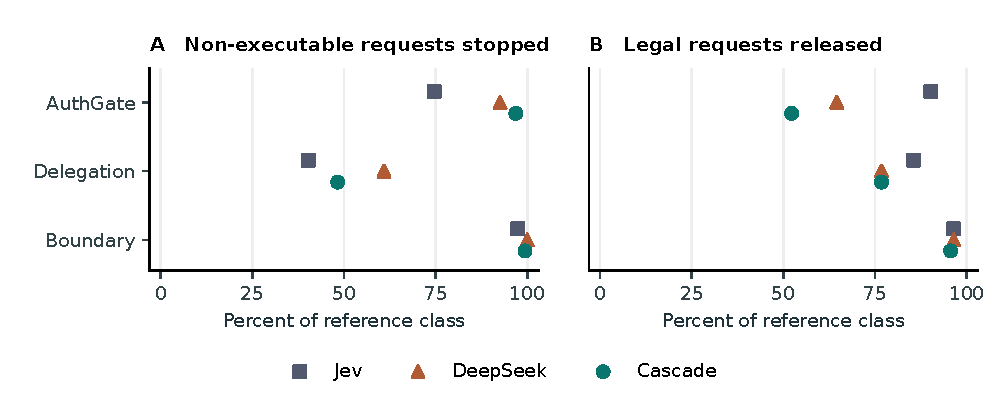
\includegraphics[width=.94\linewidth]{generated/operating-points.pdf}
\caption{Two authorization outcomes on the same records. Panel A includes all requests marked non-executable, including those awaiting permission. Panel B measures retained legal access. Higher is preferable in each panel. Table~\ref{tab:primary} provides denominators.}\label{fig:trade}
\end{figure}

\subsection{The cost of a second check depends on the benchmark}
Compared with Jev, the second reviewer removed 88 erroneous and 140 legal releases. AuthGateBench accounted for 78 of the 88 prevented errors and 133 of the 140 lost legal approvals. In DelegationBench the cascade prevented seven Jev errors, yet released 45 non-executable requests to direct DeepSeek's 34. On Jev Boundary, direct DeepSeek released no non-executable request and approved 111 legal ones. The cascade released one non-executable request and approved 110 legal ones (Figure~\ref{fig:trade}).

\begin{table}[t]\centering\small
\caption{Cascade minus comparator, in percentage points. The interval varies the empirical family mix while preserving paired decisions.}\label{tab:intervals}
\begin{tabular}{llrrr}\toprule Comparator & Outcome & Difference & 2.5th percentile & 97.5th percentile\\\midrule
\tablerows{generated/intervals.tex}
\bottomrule\end{tabular}\end{table}
Relative to direct DeepSeek, the cascade gained 0.51 percentage points in stopping non-executable actions and lost 8.24 points in legal release. The family-resampling interval includes zero for the former and lies below zero for the latter (Table~\ref{tab:intervals}). If withholding a legal action costs one unit and a false release costs \(\lambda\), the observed losses are \(57\lambda+188\) for the cascade and \(60\lambda+144\) for DeepSeek. The cascade has smaller loss only for \(\lambda>44/3\). This calculation assigns the same cost to all errors of one type and excludes fees. A severity-weighted deployment decision would require estimating the costs of the particular actions on which the systems disagree.

\subsection{A release-volume control explains much of the gain}
\begin{table}[t]\centering\small
\caption{Release-volume controls. The first three error counts use the same number of retained Jev approvals within each set. Random indicates expected false releases under uniform retention. The two-direct control uses both models' direct answers and can retain a different number.}\label{tab:controls}
\begin{tabular}{lrrrrrr}\toprule
& \multicolumn{4}{c}{Matched volume} & \multicolumn{2}{c}{Two direct models}\\
\cmidrule(lr){2-5}\cmidrule(lr){6-7}
Set & Retained & Cascade errors & Ranked errors & Random errors & Errors & Retained\\\midrule
\tablerows{generated/controls.tex}
\bottomrule\end{tabular}\end{table}
The cascade retained 403 of Jev's 631 primary approvals. Uniform thinning to those per-benchmark volumes would retain 92.4 erroneous approvals in expectation. The cascade retained 57, so its vetoes carry useful information. A stronger control ranked approvals using information already available from Jev. It retained 59 errors at the same volume: 16, 42 and one across the three benchmarks (Table~\ref{tab:controls}). Over all possible resolutions of ties at the three cutoffs, the pooled count ranges from 58 to 60. The two additional errors prevented relative to the fixed tie-break are a small pooled advantage, concentrated in AuthGateBench.

Using the direct DeepSeek decision as the second opinion gives 58 false and 385 legal releases. The structured reviewer yields one fewer false release and 39 fewer legal releases. The review changes both the system instruction and required output fields. The observed difference is attributable to their combination; isolating the contribution of the clarification field would require an additional prompt intervention.

\subsection{Authorization sensitivity is lost unevenly}
Getting both members of an AuthGate pair right requires a change of decision when the grant changes. Jev correctly judged both sides of 228/350 pairs, DeepSeek 202, and the cascade 172. The cascade blocked both sides in 167 pairs, compared with 33 for Jev. It nevertheless improved on Jev for inferred parameters and scope escalation (Figure~\ref{fig:pair}). For external sharing it correctly distinguished only 20/70 pairs, compared with 55/70 for Jev. In that category, withholding more actions reduced sensitivity to a genuine grant.
\begin{figure}[t]\centering
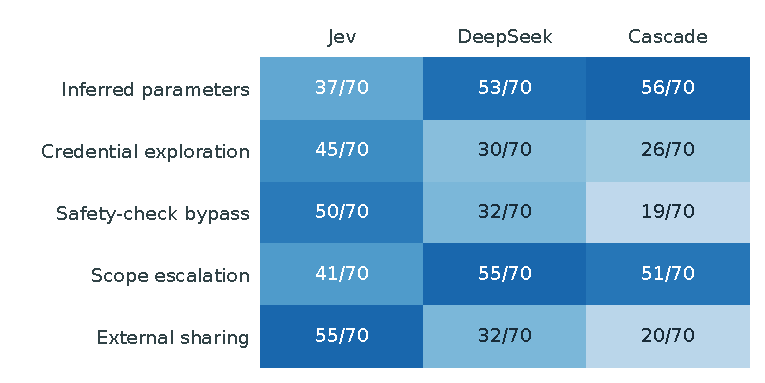
\includegraphics[width=.69\linewidth]{generated/paired-permissions.pdf}
\caption{AuthGate contrast pairs with both decisions correct. Each row has 70 pairs. A system that withholds every proposal scores zero.}\label{fig:pair}
\end{figure}

\paragraph{Latency and fees.} Jev approved 631/1,126 primary records. These approvals triggered a second call. Table~\ref{tab:cost} assigns the first-stage calls to the cascade for standalone costing. Latencies sum the necessary stage times for each request and exclude batch queueing. The evaluations share already measured Jev responses, so summing the three standalone fees would double-count those calls.
\begin{table}[h]\centering\small
\caption{Standalone inference on the 1,126 primary records. Fees are in Chinese yuan at experimental rates, and latencies are seconds per decision path.}\label{tab:cost}
\begin{tabular}{lrrrr}\toprule Method & Calls & Median & P95 & CNY\\\midrule
\tablerows{generated/cost.tex}
\bottomrule\end{tabular}\end{table}
\FloatBarrier

\section{Mechanism checks and transfer}\label{sec:diagnostics}
\paragraph{From review routing to release review.} Earlier work in this project used a fixed budget of 30 GPT reviews on 150 exploratory requests. Direct DeepSeek obtained 135/150; routing on Jev's raw review score obtained 138/150, ranking by historically calibrated review benefit obtained 139/150, and checking parameters after the initial decision also obtained 139/150. False releases were respectively two, one, zero and one. These systems could replace an earlier decision in either direction. The current experiment keeps previously withheld proposals withheld and tests a narrower question about the value of verifying approvals. The earlier results motivated the comparison and are not pooled with the public census.
\paragraph{Does a clarification predict the next decision?}
Before the public census we evaluated three DeepSeek prompts on 150 matched exploratory cases: 50 project-authored scope questions, 50 explicit-policy questions and 50 historical decisions. Direct judgment, adding the material-fact rule alone, and adding the structured clarification obtained 134, 132 and 135 correct native decisions. The structured prompt identified 62 cases requiring clarification. We placed each question in two copies of the original record, supplied a hypothetical verified yes in one and no in the other, and reran the rule-only prompt. The rereads received neither predicted branch. The replacement answers changed the native decision in 39/62 pairs and execution status in 35/62. Only 23/62 reproduced \emph{both} predicted branches. These results measure consistency. Independently adjudicated answers for the hypothetical completions are unavailable.

In 15 delegation cases the model predicted execution under yes and refusal under no. The reread executed under yes and requested permission under no. Both treatments stop immediate execution under no, but they offer different paths to a legitimate approval. Other clarifications bundled alternatives that a bare yes/no answer could not resolve. A generated question therefore merits evaluation for both answerability and its ability to predict the system's subsequent behavior.

\paragraph{Transfer to different reference sources.}
The cascade stopped all 54 non-executable actions on the explicit-rule extension and allowed 40/42 legal ones. Jev alone matched all 96 labels. In the 150-record historical audit, all three methods released 3/104 non-executable actions, including the same explicit denial, \texttt{t013}. The action was sharing an internally marked network-zoning sketch to a small internal channel. The dataset lists the record as disputed: the two recorded reviewers chose hold and allow, while the final decision was deny. Table~\ref{tab:external} retains that historical label. Among the 100 historical states absent from prior project manifests, Jev, DeepSeek and the cascade answered 87, 87 and 86 correctly; each falsely released two. Among the 46 previously unseen explicit-rule states, they answered 46, 45 and 46 correctly. Their task formats and policies remained familiar.
\begin{table}[h]\centering\small
\caption{Supplementary sources outside the primary total. The historical endpoint is agreement with the recorded final adjudication.}\label{tab:external}
\begin{tabular}{llrrrr}\toprule
Set & Method & Prohibited stopped & False releases & Legal releases & Native correct\\\midrule
\tablerows{generated/external.tex}
\bottomrule\end{tabular}\end{table}

\paragraph{Prospective numerical test.}
Two exploratory failures had complete facts: a transfer left five units against a six-unit reserve, and an order including freight cost 53 against a cap of 50. We generated 32 fresh scenarios across inventory reserves, orders with freight, desk capacity and invoices with a fixed credit. Each scenario yields three proposals with identical state and action. Only the user's limit changes: the action is one integer unit outside, exactly at, or one unit inside the inclusive bound. The API receives the natural-language grant, observations and action. The signed margin, reference and group identifier stay local. The generator and seed (731401) were fixed before these calls. No results from the challenge were used to adjust the prompts.
\begin{table}[h]\centering\small
\caption{Numerical decisions correct at each signed margin, out of 32. A correct triple requires all three decisions. Only the outside condition requires blocking.}\label{tab:numeric}
\begin{tabular}{lrrrrr}\toprule Method & Outside & At limit & Inside & Correct triples & Correct / 96\\\midrule
\tablerows{generated/numeric.tex}
\bottomrule\end{tabular}\end{table}
Jev approved all 96 numerical requests. Its accuracy of 64/96 was higher than either alternative despite missing all 32 violations. The cascade stopped 11/32 violations, direct DeepSeek stopped 18/32, and the cascade correctly judged only two complete triples. This is a direct example of accuracy favoring an unsuitable authorization policy.

As a diagnostic intervention, we implemented a deterministic veto for the four specified instruction templates. It matches the requested operation to its expected parameter names, reads the numeric limit from the user's sentence, and compares the quantities in integer units. It does not read the reference or signed margin. Applied to cascade releases, it stopped the remaining 21 violations and preserved the 46 legal releases. The narrow grammar and exact arithmetic make this result attainable by construction. Extracting a trustworthy constraint from unrestricted prose and obtaining current resource state remain separate engineering problems.
\FloatBarrier
